%%________________________________________________________________________
%% LEIM | PROJETO
%% 2022 / 2013 / 2012
%% Modelo para relatório
%% v04: alteração ADEETC para DEETC; outros ajustes
%% v03: correção de gralhas
%% v02: inclui anexo sobre utilização sistema controlo de versões
%% v01: original
%% PTS / MAR.2022 / MAI.2013 / 23.MAI.2012 (construído)
%%________________________________________________________________________


%%________________________________________________________________________
\chapter{Introdução}
\label{ch:introducao}
%%________________________________________________________________________

No contexto do ensino superior, tem-se dado cada vez mais importância à integração de ferramentas tecnológicas que tornem o processo de aprendizagem mais prático, como é o caso do simulador utilizado pelos alunos do \gls{iscal}. Esta ferramenta permite que os estudantes apliquem, de forma interativa, os conhecimentos adquiridos ao longo do curso, colocando-os em situações de tomada de decisão semelhantes às que enfrentariam num ambiente real. Deste modo, o simulador não só reforça os conteúdos teóricos, como também reforça o desenvolvimento das competências aprendidas. 

Neste contexto, a análise eficiente de dados (da plataforma de simulação) torna-se essencial para a tomada de decisões estratégicas e tem impacto na avaliação final dos alunos, no entanto, a complexidade e a falta de uma ferramenta visual que ajude a perceber as informações apresentadas pela plataforma de simulação podem representar um desafio grande para os estudantes.

\section{Motivação}
O presente projeto surgiu da necessidade  entre os alunos do \gls{iscal} que utilizam o simulador \textit{Marketplace Simulations - International Corporate Management}, que é um simulador de negócios internacionais e que iremos descrever no capítulo seguinte, onde os alunos se agrupam em empresas fictícias e simulam a criação de um negócio num mercado internacional. Embora a plataforma apresente toda a informação necessária à tomada de decisões na simulação, esses dados estão dividos em múltiplas secções e apresentados em tabelas, com poucas funcionalidades de visualização. Esta limitação obriga os alunos a alternar entre páginas, copiar dados manualmente e criar folhas de cálculo externas, comprometendo a eficiência e a análise da informação.

\section{Objetivos}

A aplicação proposta neste relatório pretende ajudar nesse sentido, oferecendo uma interface que permite aos utilizadores carregar dados retirados da plataforma de simulação e tornar esses ficheiros em visualizações que podem ser consultadas e manipuladas. A aplicação permitirá aos utilizadores:

\begin{itemize}
    \item Criar uma conta na plataforma que permita persistir a informação carregada.
    \item Carregar ficheiros exportados da plataforma de simulação;
    \item Visualizar os dados em gráficos interativos;
    \item Conseguir ter uma experiência de utilização intuitiva e fácil;
\end{itemize}

Do ponto de vista técnico, queremos que a aplicação adote uma arquitetura fácil de manter e que vá de encontro à utilização da plataforma, dando importância aos seguintes itens:
\begin{itemize}
    \item A normalização e transformação automática de dados provenientes de fontes externas;
    \item A facilidade na gestão de ficheiros, com o objetivo de oferecer uma interface fácil para os utilizadores finais.
    \item Organizar a informação por utilizador, garantindo que o utilizador apenas consegue consultar a informação carregada.
    \item Adotar um modelo de funcionamento semelhante à plataforma de simulação, de modo a tornar a experiência de utilização mais intuitiva e garantido que a nossa aplicação tenha fronteiras claras de utilização.
\end{itemize}

Ao longo deste relatório, serão detalhadamente apresentadas as decisões tomadas, bem como os fundamentos que orientaram o desenvolvimento da aplicação proposta.

%%________________________________________________________________________
\chapter{Trabalho Relacionado}
\label{ch:trabalhoRelacionado}
%%________________________________________________________________________

O presente projeto insere-se num contexto mais geral de ferramentas pedagógicas e \gls{sad}, ainda que neste caso concreto, em ambientes simulados no ensino superior. No âmbito do \gls{iscal}, a utilização da plataforma \textit{Marketplace Simulations} e permite aos estudantes desenvolver competências práticas em ambientes virtuais de negócios, simulando o funcionamento de mercados reais. A necessidade de suporte digital à análise e simulação motivou o desenvolvimento de outras ferramentas auxiliares, com destaque para um projeto também realizado em parceria com o \gls{iscal}, focado em simulações parciais de modelos económicos.

Esse projeto, embora partilhe uma motivação semelhante, segue uma abordagem distinta. Em particular, a aplicação permite simular cenários específicos com base em inputs manuais, o que pode ser útil para quando se procura prever resultados com foco muito concreto (por exemplo, simular o impacto de uma única variável nos resultados). A nossa plataforma foca-se numa outra vertente, em que pretende ser uma ferramenta para auxiliar o ensino de forma prática.

O nosso projeto assume então o uso de dados extraídos diretamente da plataforma de simulação, e a valorização da experiência do utilizador na apresentação de dados. 

%%________________________________________________________________________
\chapter{Modelo Proposto}
\label{ch:modeloProposto}
%%________________________________________________________________________

(falta introduzir o modelo proposto)


%%________________________________________________________________________
\section{Requisitos}
\label{sec:requisitos}
%%________________________________________________________________________

\subsubsection{Requisitos funcionais}
Os requisitos funcionais descrevem as funcionalidades específicas que a aplicação deve oferecer para atender às necessidades dos utilizadores. No contexto deste projeto, definem as ações que o sistema deve ser capaz de executar. No nosso projeto, identificamos os seguintes requisitos, ordenados por prioridade:

\begin{itemize}
    \item \textbf{Visualização de dados:} os utilizadores devem poder visualizar gráficos interativos baseados nos dados carregados, com a possibilidade de aplicar filtros como país ou quarter selecionado.

    \item \textbf{Gestão de ficheiros:} os utilizadores devem poder carregar ficheiros, associá-los a quarters e eliminá-los quando necessário. O sistema valida os formatos e garante que apenas ficheiros válidos são processados.
    
    \item \textbf{Gestão de quarters:} cada utilizador pode criar períodos identificados como \textit{Quarter N}, para organizar os ficheiros carregados. Tem também de ser possível visualizar a lista de quarters disponíveis.

    \item \textbf{Autenticação:} o sistema deve permitir a criação de contas e o login por parte dos utilizadores, garantindo que cada um acede apenas aos seus próprios dados.
    
\end{itemize}

\subsubsection{Requisitos não funcionais}

Alguns requisitos não funcionais foram igualmente críticos para garantir a robustez e usabilidade do sistema. Os requisitos identificados foram os seguintes:

\begin{itemize}
    \item \textbf{Usabilidade:} a interface deve ser intuitiva, suportar múltiplos browsers e permitir o carregamento progressivo de gráficos sem bloquear a interação do utilizador (\textit{lazy load}).
    
    \item \textbf{Segurança:} o sistema deve garantir uma autenticação segura e assegurar que cada utilizador ou grupo apenas consegue aceder aos seus próprios dados. Deve também assegurar que só permite carregar ficheiros com o formato previsto.
    
    \item \textbf{Performance:} a aplicação deve ser capaz de suportar múltiplos utilizadores em simultâneo sem degradação significativa, mantendo uma resposta rápida às interações.
    
    \item \textbf{Acessibilidade:} o sistema deve ser acessível por teclado e compatível com leitores de ecrã (\textit{screen-reader friendly}).

    \item \textbf{Normalização de dados:} os dados extraídos dos ficheiros devem ser automaticamente normalizados para garantir consistência e compatibilidade com o sistema de visualização.

\end{itemize}

Os tabelas de requisitos por inteiro estão incluidas em apêndice (\cf, capítulo \ref{ch:tabRequisitos}).

\section{Casos de Utilização}

Com base nos requisitos funcionais e não funcionais identificados na secção anterior, foram definidos os casos de utilização que iremos suportar. O diagramas correspondente, tal como a matriz de prioridade, encontram-se no (\cf, capítulo \ref{ch:casosUtilizacao}), mas em resumo, os casos de utilização são os que se seguem:

\begin{enumerate}
    \item \textbf{Registo de utilizador: } \\
    O utilizador acede à plataforma pela primeira vez e opta por criar uma conta. O sistema solicita os dados de autenticação e valida se o utilizador já existe. Caso não exista, a conta é criada e o utilizador é autenticado automaticamente. \\
    \textit{Este caso responde ao requisito funcional de autenticação e está alinhado com os requisitos não funcionais de segurança.}
    
    \item \textbf{Autenticação do utilizador: } \\
    Ao entrar na aplicação, o utilizador introduz o seu username e password. O sistema valida o login com base nos dados guardados e, se for bem-sucedido, redireciona o utilizador para a página principal. \\
    \textit{Relaciona-se com os requisitos de segurança e experiência de utilizador.}
    
    \item \textbf{Criação de um quarter: } \\
    O utilizador, já autenticado, pode criar um novo quarter, identificando-o por um número. O sistema garante que esse número é único para o utilizador. \\
    \textit{Este caso de utilização reflete o requisito funcional de organização por quarters, e está diretamente ligado à estrutura de dados definida no modelo.}
    
    \item \textbf{Carregamento de ficheiros: } \\
    O utilizador escolhe um quarter e carrega ficheiros exportados da plataforma de simulação. O sistema valida a extensão, processa os ficheiros, aplica a pipeline de normalização para cada folha do Excel. Os dados serão associados ao quarter de onde foram criados. \\
    \textit{Este caso é central no sistema e concretiza os requisitos de Carregamento, normalização dos dados, e compatibilidade com os ficheiros da plataforma Marketplace Simulations.}

    \item \textbf{Eliminação de ficheiros: } \\
    O utilizador pode eliminar ficheiros previamente carregados. O sistema remove as referências no backend, marca os ficheiros antigos como inativos e evita que continuem a ser usados na geração dos gráficos. \\
    \textit{Este caso garante a gestão de dados pelo utilizador e reforça o princípio de manter apenas uma versão ativa por ficheiro.}
    
    \item \textbf{Visualização de gráficos: } \\
    Após carregar os ficheiros, o utilizador pode aceder a gráficos criados a partir dos dados normalizados. Os gráficos são interativos, e o utilizador pode aplicar filtros (por exemplo, selecionar o país ou o quarter atual) para ajustar a visualização. Apenas os ficheiros mais recentes são utilizados para construir os gráficos. \\
    \textit{Este caso corresponde ao requisito de visualizações interativas e integra a lógica de isolamento de dados, performance e usabilidade.}
    
\end{enumerate}

Com os casos de utilização estabelecidos, foram identificados então os requisitos da plataforma, que podemos separar em requisitos funcionais e não funcionais.

%%________________________________________________________________________
\section{Fundamentos}
\label{sec:fundamentos}


\subsection{Marketplace Simulations}

A Marketplace Simulations  é uma empresa que desenvolve plataformas de simulação para fins educativos, ou seja, ferramentas que colocam os estudantes numa espécie de jogo onde cada equipa gere a sua própria empresa e compete com os colegas em cenários simulados. Acaba então por funcionar como uma espécie de laboratório virtual que pode ser usado no ensino superior, como no \gls{iscal}, onde os alunos aplicam os conceitos aprendidos numa experiência em contexto educativo.

No caso concreto do nosso projeto, a aplicação em questão chama-se International Corporate Management (referida doravante como plataforma de simulação) \cite{MarketplaceSim_2025}, e é utilizado tipicamente no último semestre, na cadeira Projeto de Simulação em Negócios Internacionais da Licenciatura de Comércio e Negócios Internacionais \cite{FUC_ISCAL_2025}. 

\begin{figure}[h]
    \centering
    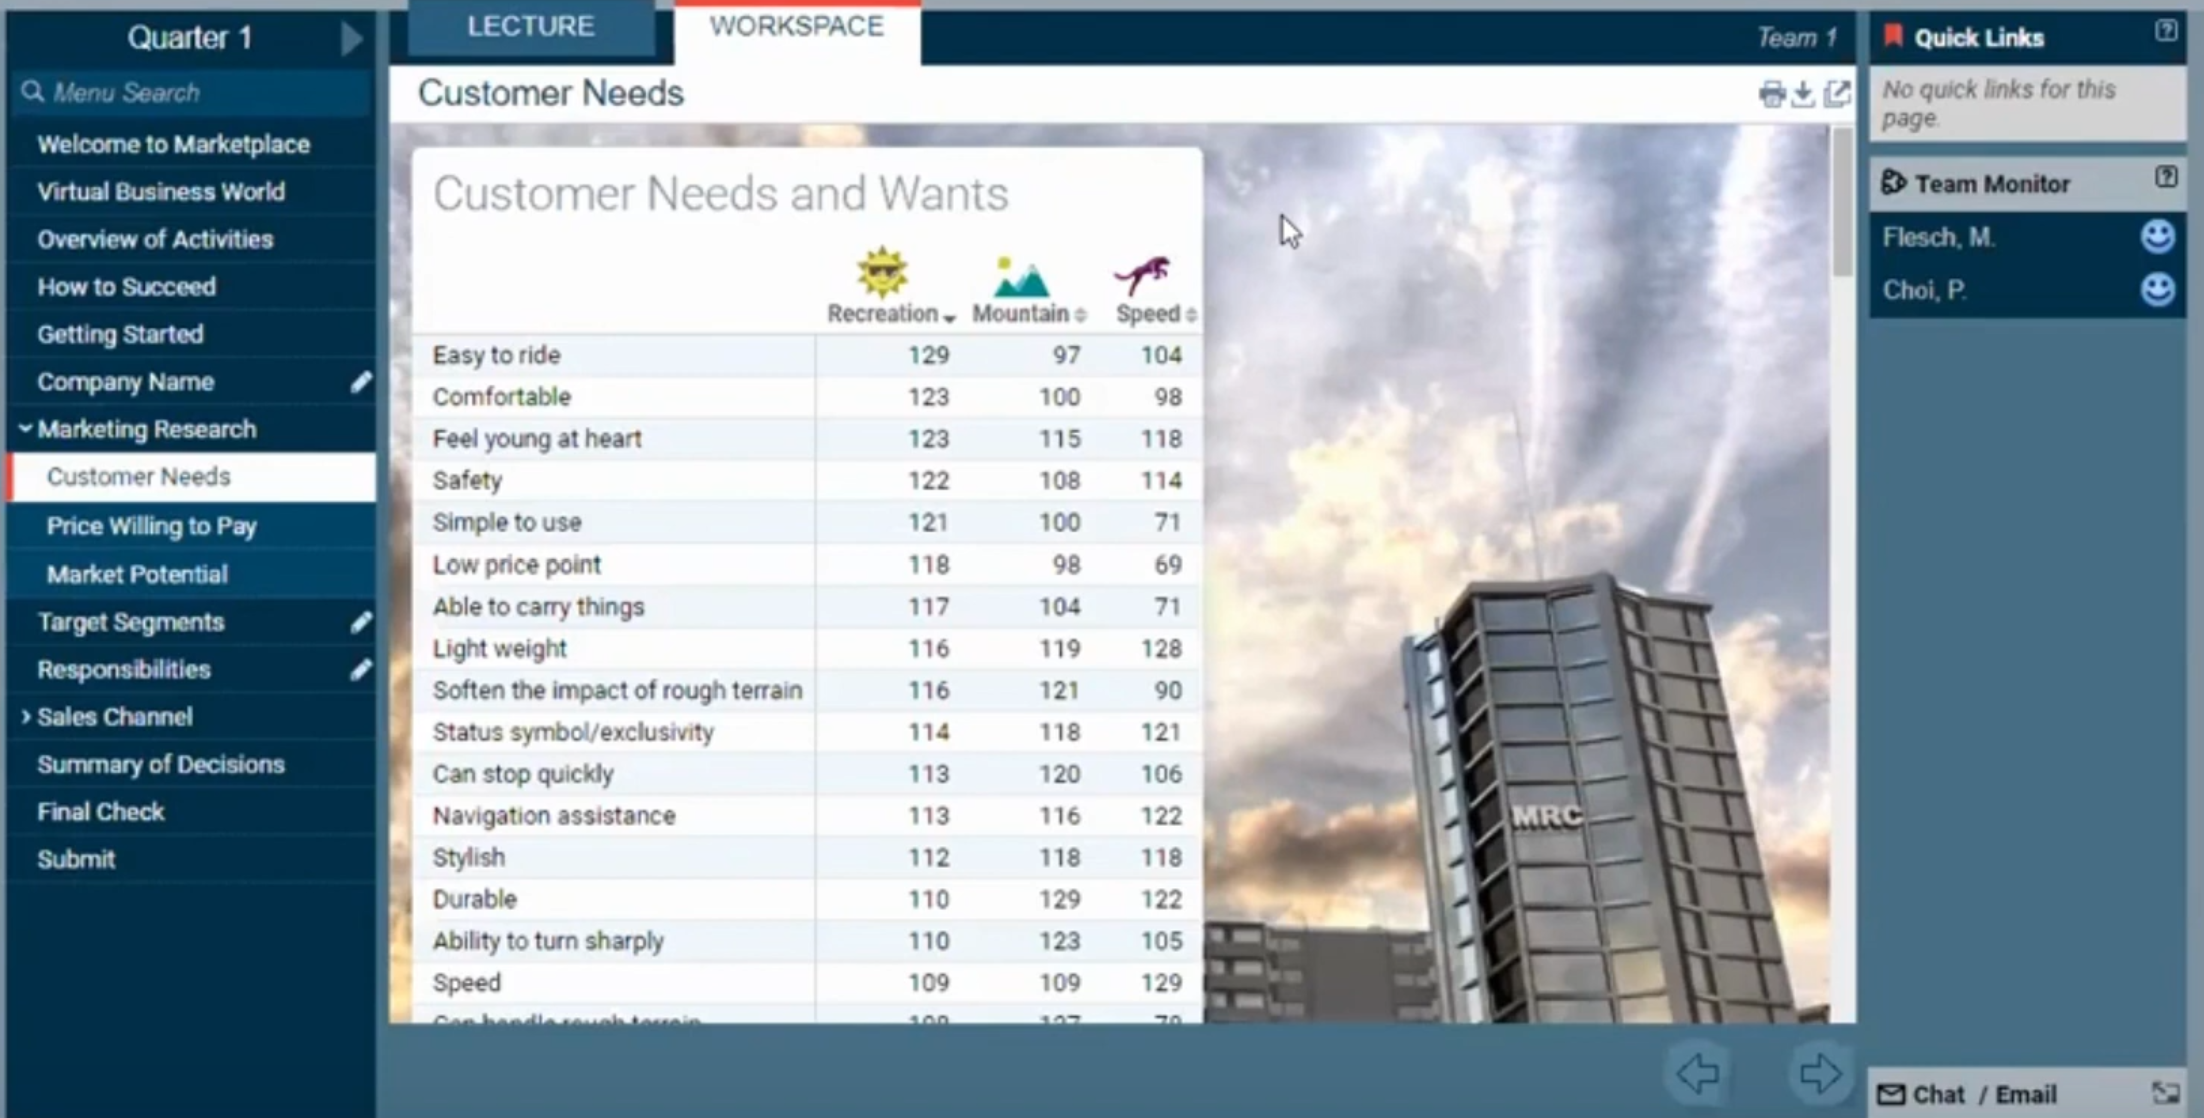
\includegraphics[width=\textwidth]{./img/marketplace1}
 \caption{Captura de ecrã da aplicação International Corporate Management}
 \end{figure}

Aqui, cada grupo de alunos representa uma empresa que tem de atuar num mercado internacional, tomando decisões sobre o posicionamento de produto, investimento, preços, distribuição, entre outras opções. Essas decisões são processadas pela plataforma, que simula o comportamento do mercado com base num algoritmo interno. 

A cadência da simulação é dada por quarters, que representam uma semana simulada. No final de cada quarter, os alunos recebem os dados com os resultados das decisões anteriores, o que obriga a uma análise comparativa constante entre períodos. É precisamente esta ciclo, decidir, analisar, ajustar, repetir, que dá ritmo à simulação e aproxima o exercício de uma situação real.

Para a análise, os alunos têm à disposição os dados, na plataforma,  nas várias secções disponiveis que na sua maioria são apresentados em tabelas, o que faz com que os alunos saltem entre secções, ou tenham de fazer gráficos à mão ou em ultimo caso, extrair a informação da plataforma. 

\subsection{Sistemas de apoio à decisão}
\label{sec:sad}
Um \gls{sad} é uma aplicação ou conjunto de aplicações projetadas para ajudar os utilizadores a tomar decisões mais informadas e fundamentadas, geralmente com base na análise de dados. Na prática, um \gls{sad} recolhe, organiza e processa dados, e apresenta esses dados de forma visual (como gráficos), permitindo aplicar filtros e explorar cenários. Ou seja, não toma decisões por si só, mas fornece os elementos certos para que o utilizador possa decidir melhor, especialmente em contextos complexos ou com muitos dados.


\subsection{Backend e Frontend}

O projeto desenvolvido segue uma arquitetura de aplicações web, dividida em duas grandes camadas: \textit{backend} e \textit{frontend}.

O \textit{backend} corresponde à "parte invisível" da aplicação, é o lado do servidor, responsável por tratar os dados, executar "lógica de negócio" e responder aos pedidos feitos pelos utilizadores. No contexto deste projeto, o \textit{backend} é responsável por funcionalidades como o carregamento de ficheiros, processamento e normalização dos dados,  autenticação e a disponibilização desses dados através de uma API.

O \textit{frontend}, por outro lado, é a "parte visível" da aplicação, é o que o utilizador vê e com o que interage diretamente no \textit{browser}. Inclui os formulários, gráficos e outros elementos criados a partir dos dados processados.

Esta separação entre \textit{backend} e \textit{frontend} facilita a manutenção do sistema e permite que ambas as partes evoluam de forma independente, podendo até ser substituídas sem necessidade de reescrever o sistema completo.

As tecnologias utilizadas para o desenvolvimento serão descritas no capítulo \ref{ch:tecnologias}.

\subsection{Tipos de gráficos}

Durante a análise que fizemos foram selecionados diferentes tipos de gráficos, de acordo com o tipo de análise que cada conjunto de dados pretendia suportar. Cada tipo de gráfico foi escolhido com base na sua capacidade de representar visualmente os dados e a sua facilidade de interpretação.

\textbf{Gráfico de Barras (Bar Chart):}
Este tipo de gráfico foi utilizado para comparar valores entre diferentes categorias, como marcas, cidades ou segmentos de mercado. A disposição visual das barras permite uma leitura rápida das diferenças de desempenho entre categorias, sendo util para dados que não são temporais. Foram usadas variantes como barras empilhadas e barras agrupadas, dependendo da granularidade pretendida.

\begin{figure}[H]
\centering
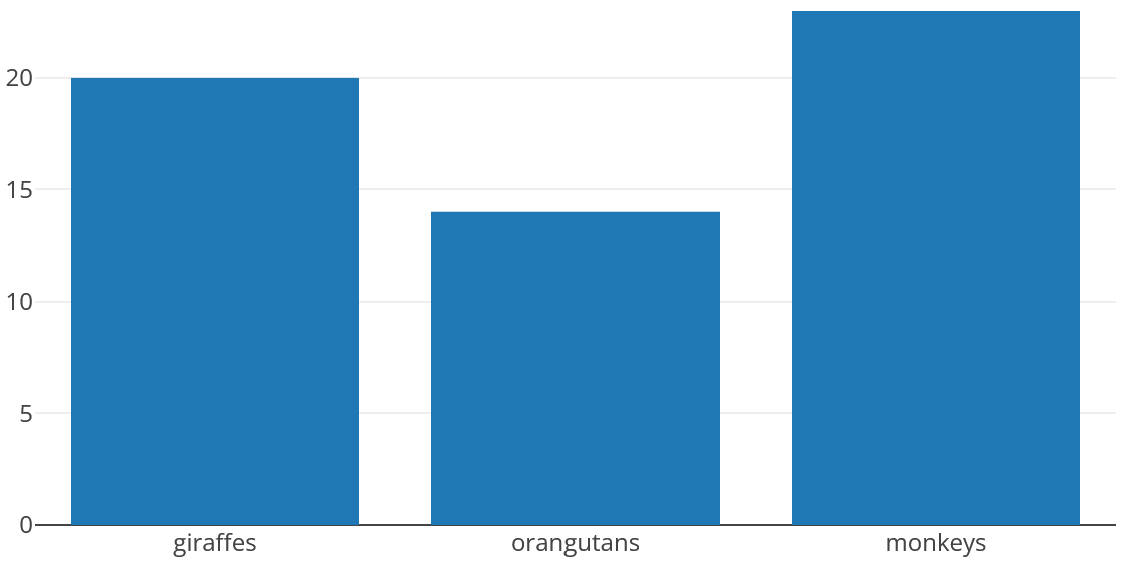
\includegraphics[max width=12cm, keepaspectratio]{./img/barras1}
\caption{Exemplo de gráfico de barras}
\end{figure}
\noindent

\begin{figure}[H]
\centering
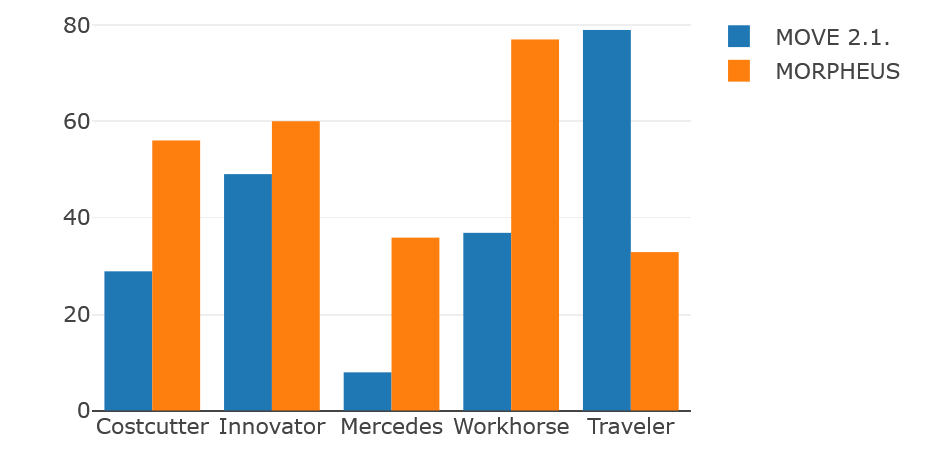
\includegraphics[max width=12cm, keepaspectratio]{./img/agrupada}
\caption{Exemplo de gráfico de barras agrupadas}
\end{figure}
\noindent

\begin{figure}[H]
\centering
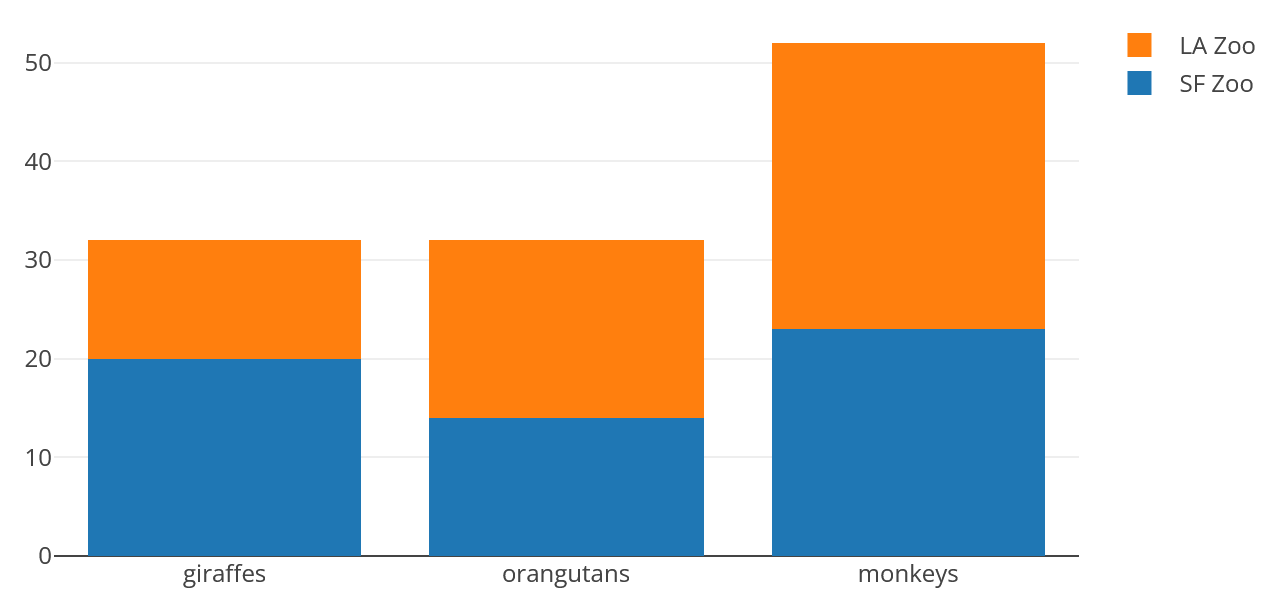
\includegraphics[max width=12cm, keepaspectratio]{./img/empilhada}
\caption{Exemplo de gráfico de barras empilhadas}
\end{figure}
\noindent

\textbf{Gráfico de Sectores (Pie Chart):}  
Utilizado para representar distribuições percentuais, como a repartição de dados por segmento. Este tipo é  intuitivo para visualizar como uma totalidade se divide entre diferentes partes, sendo adequado para dados onde se pretendia enfatizar proporções relativas (como por exemplo dados categorizados por segmentos)

\begin{figure}[H]
    \centering
    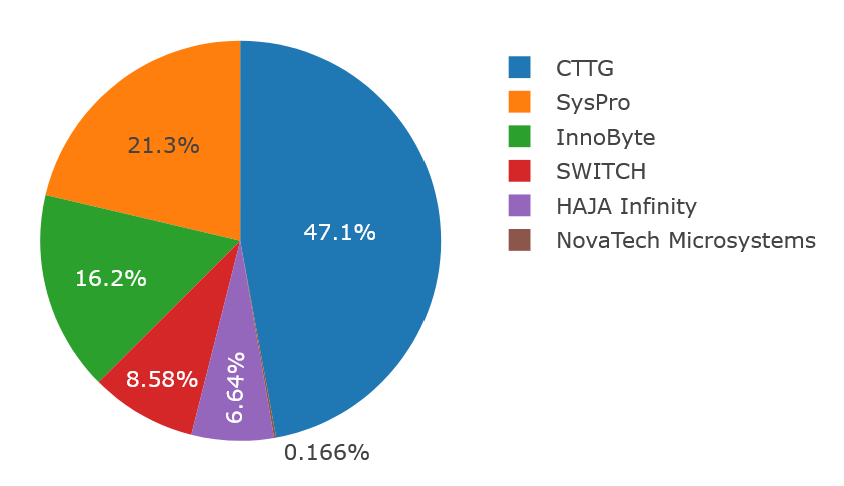
\includegraphics[max width=12cm, keepaspectratio]{./img/pie}
    \caption{Exemplo de gráfico de sectores}
\end{figure}
\noindent

\textbf{Gráfico Financeiro (Waterfall Chart):}  
Empregado especificamente para representar balanços financeiros, como resultados acumulados de receitas e despesas. O gráfico cascata” (waterfall) permite visualizar como diferentes contribuições individuais afetam um valor final, facilitando a análise de ganhos e perdas ao longo do tempo ou de processos financeiros.

\begin{figure}[H]
    \centering
    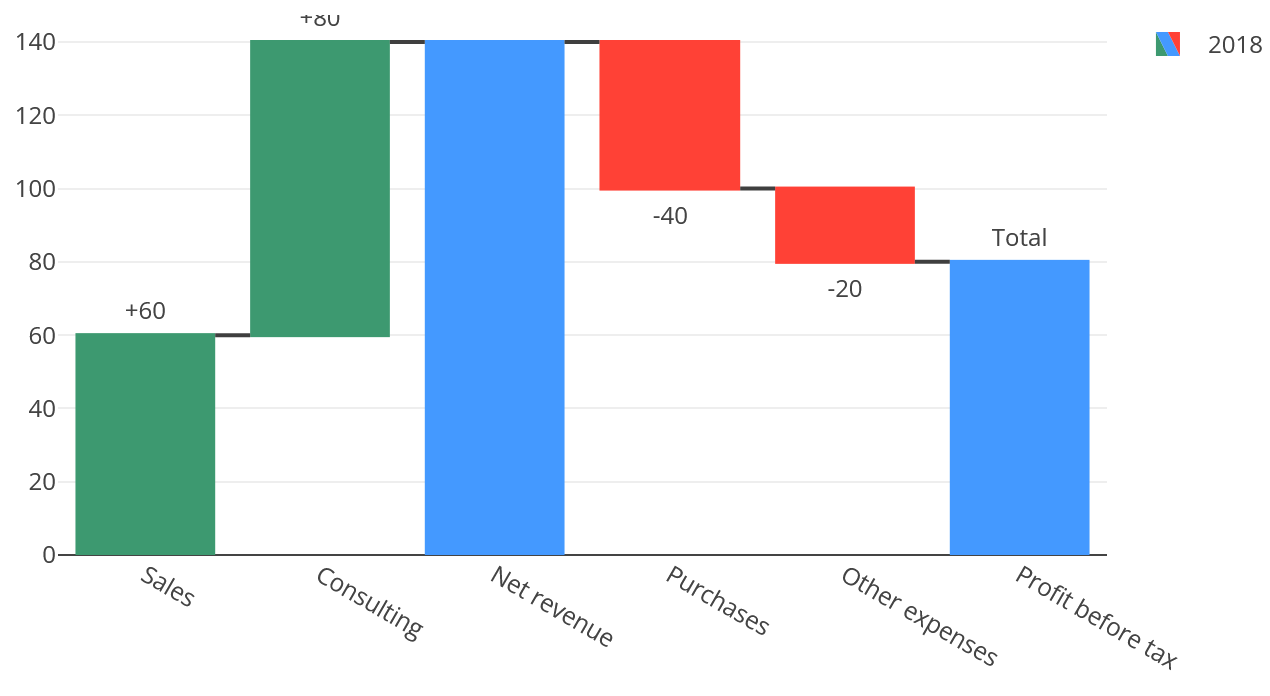
\includegraphics[max width=12cm, keepaspectratio]{./img/waterfall}
    \caption{Exemplo de gráfico financeiro}
\end{figure}
\noindent

\textbf{Diagrama de Quartis (Box Plot):}
Os diagramas de quartis, foram utilizados para representar dados que eram distribuições, permitindo visualizar de forma rápida a mediana, os quartis e possíveis valores extremos. Este tipo de diagrama é util para comparar a diferença entre diferentes categorias, como por exemplo comparar a dispersão de vendas entre várias marcas ou cidades. A interpretação deste tipo de visualização exige um conhecimento prévio de conceitos estatísticos como mediana e quartis, o que pde dificultar a leitura para o público-alvo, mas que simplifica a representação dos dados.

\begin{figure}[H]
    \centering
    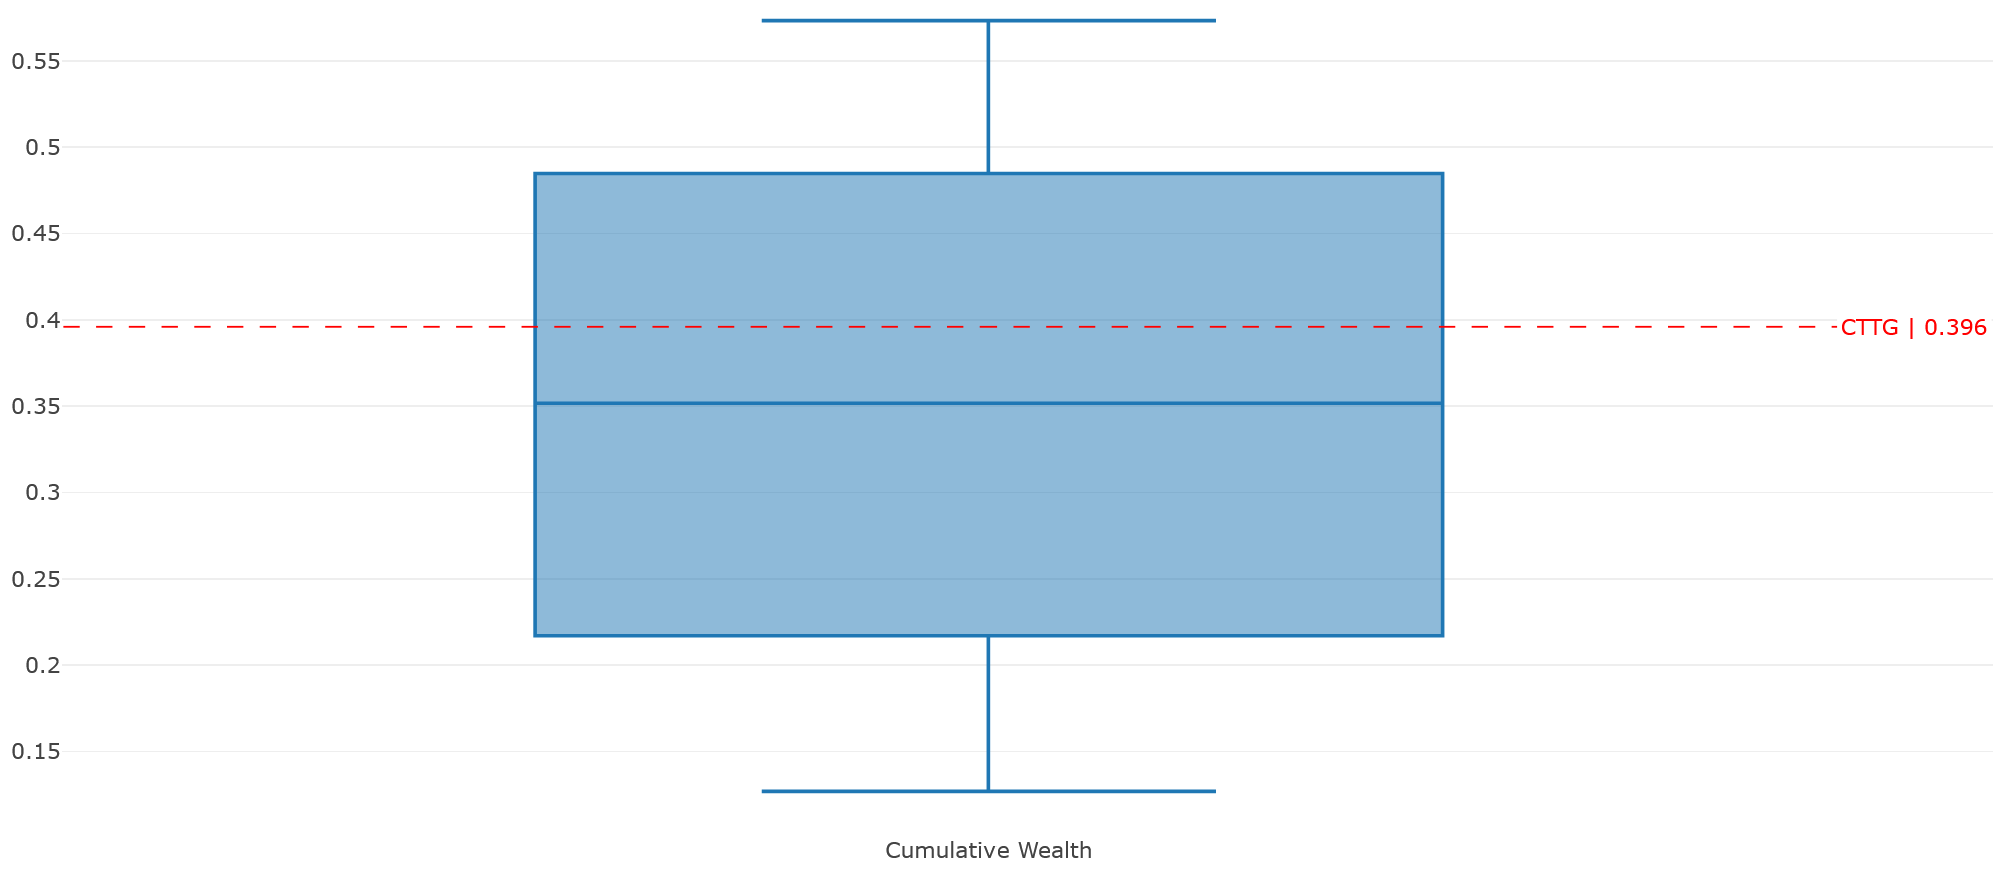
\includegraphics[max width=12cm, keepaspectratio]{./img/box}
    \caption{Exemplo de Diagramas de Quartis}
\end{figure}
\noindent

\textbf{Diagrama de Sankey (Sankey Diagram):}
Os diagramas de Sankey são utilizados para representar fluxos entre diferentes categorias, destacando a quantidade transferida de uma categoria para outra. Estes diagramas são particularmente úteis para ilustrar a passagem de clientes entre necessidades ou segmentos. Cada fluxo é representado por uma linha cuja largura é proporcional à quantidade movida, permitindo uma visualização intuitiva da importancia dos fluxos. Para evitar representações complexas, decidimos apenas recorrer a este tipo apenas quando os dados não poderiam ser representados de outra forma, ou tratados de forma a simplificar a representação.

\begin{figure}[H]
    \centering
    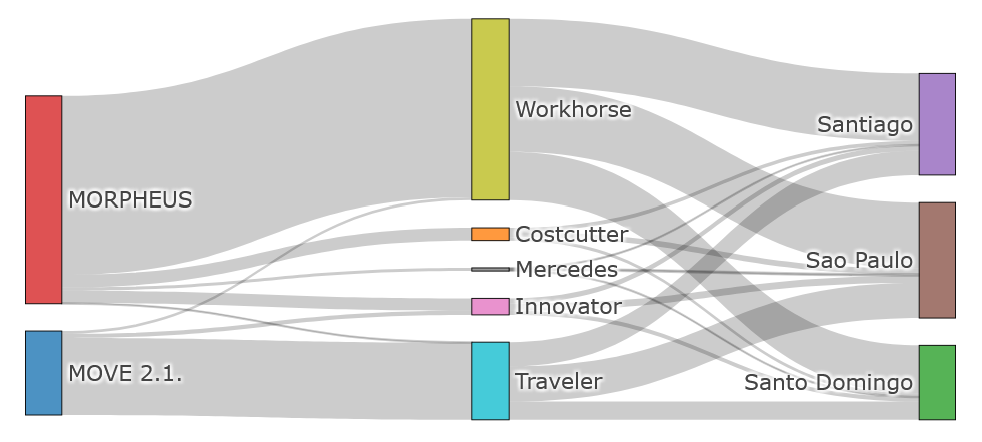
\includegraphics[max width=12cm, keepaspectratio]{./img/skankey}
    \caption{Exemplo de gráfico de Sankey}
\end{figure}
\noindent

Outros tipos de gráficos relevantes para o projeto, mas que não foram utilizados foram:

\textbf{Gráfico de Linhas (Line Chart):}  
Escolhido para representar séries temporais, como a evolução de vendas ou de quotas ao longo de vários trimestres. As linhas permitem identificar tendências e variações. No nosso projeto, não tivemos necessidade de usar este tipo uma vez que nenhum dos dados recebidos era relativos a séries temporais, pelo que a sua utilização não era intuitiva para os utilizadores.

\textbf{Gráfico de Radar (Radar Chart):}  
Utilizado para comparar múltiplas variáveis em relação a um valor comumn, como no caso da avaliação de diferentes necessidades dos clientes em simultâneo. Este tipo de gráfico permite identificar rapidamente pontos fortes e fracos em várias dimensões de análise. Apesar destas vantagens, nos dados que recebemos não conseguimos identificar utilizações onde este tipo de gráfico beneficiasse os utilizadores finais.

\textbf{Gráfico de Dispersão (Scatter Plot):}
Os gráficos de dispersão foram considerados para representar relações entre duas variáveis quantitativas, como por exemplo entre o preço e a procura de determinados produtos. Cada ponto no gráfico representa uma observação individual, permitindo identificar padrões de correlação (positiva, negativa ou inexistente) entre variáveis. No nosso caso, consideramos utilizar um tipo especifico de gráfico de dispersão (gráfico de dispersão num mapa) mas a leitura tornou-se confusa, uma vez que era pouco legivel para alunos, e não considerava localizações ficticias.
\end{itemize}

A escolha dos tipos de gráficos teve como objetivo manter a clareza e facilidade da informação e permitir diferentes leituras sobre os dados extraídos. Cada gráfico foi pensado para às características das categorias disponíveis, considerando tanto a o formato dos dados (quantitativa ou categórica) como o objetivo da análise (comparação, distribuição, evolução ou composição).

%%________________________________________________________________________
\section{Abordagem}
\label{sec:abordagem}
%%________________________________________________________________________

O projeto proposto pretende então ajudar nesse sentido, de conseguir transformar dados desta plataforma em algo mais fácil e rápido de analisar. Tento o contexto da plataforma, iremos então descrever duas abordagens que considerámos.

\subsection{Web Scraping}
A primeira abordagem que consideramos foi a hipótese de automatizar a extração dos dados diretamente da plataforma do Marketplace Simulations, através de técnicas de web scraping. A ideia parecia interessante numa fase inicial, já que permitiria reduzir a dependência do utilizador no processo de exportação  dos dados. No entanto, rapidamente percebemos que esta abordagem trazia vários desafios que, na prática, a tornavam pouco viável, ou mesmo arriscada.

Primeiro, cada conta na plataforma está associada a um grupo de alunos, ou seja, é uma conta ativa e única, usada diretamente durante a simulação. Isto significa que qualquer processo automático que iniciasse sessão, mesmo que fosse só para leitura, poderia de forma acidental interagir com a interface e acabar por alterar alguma opção, o que não seria bom para os alunos porque podia afetar a sua avaliação final. Além disso, como o acesso à plataforma é feito por licenças pagas, não existe qualquer possibilidade de criar uma conta de serviço ou utilizador apenas para leitura. Ou seja, qualquer tentativa de scraping teria de reutilizar credenciais reais, o que levanta não só questões de segurança, mas também (possivelmente) legais, uma vez que a plataforma pode não permitir o scraping

Outro fator que influenciou a nossa decisão foi o próprio risco técnico do scraping: plataformas deste tipo estão muitas vezes protegidas com mecanismos contra automação (como por exemplo ecrãs CAPTCHA), e não conhecendo em detalhe a aplicação, poderíamos facilmente encontrar esse tipo de proteções, que são difícies de automatizar.

Pelos motivos acima, optámos por não seguir esta abordagem. Em vez disso, definimos como parte da utilização da nossa aplicação que os próprios alunos devem exportar dados a partir da plataforma de simulação e carregar para a nossa aplicação. Esta solução, embora mais manual, garante segurança, respeita a integridade das contas dos utilizadores, e evita problemas legais ou técnicos com a aplicação de simulação.

\subsection{Exportação e carregamento manual de ficheiros}

A abordagem que acabamos por usar foi os alunos exportam manualmente os dados diretamente da plataforma de simulação e carregarem esses ficheiros na nossa plataforma. A partir daí, o sistema processa e normaliza os dados recebidos, e mostra gráficos com base nesses dados. Esta abordagem, apesar de requerer uma ação manual do lado do utilizador, é mais segura que a alternativa de web scraping, pelos os motivos apresentados acima. Deste modo, garantimos um equilíbrio entre usabilidade, segurança e fiabilidade do sistema. Acabamos então por criar um \gls{sad} (\cf, capítulo \ref{sec:sad}) que permita os estudantes tomarem melhores decisões.

Com esse objetivo, procurámos que a nossa aplicação refletisse a estrutura da própria simulação. Como tal, os dados são organizados por quarters, como acontece na plataforma de simulação e permitir o carregamento dos dados exportados. Estes ficheiros são depois processados o que nos permite trabalhar com dados mais consistentes. 

Esta estrutura base implica a existência de três entidades principais na nossa aplicação (que iremos descrever nos capítulos seguintes) e cuja interação define  o funcionamennto do sistema.


\subsubsection{\textit{Quarters}}

Os quarters funcionam como \textit{buckets} para organizar os ficheiros carregados pelos utilizadores. Cada utilizador pode criar múltiplos quarters, identificados de forma única por um número.

O propósito em incluir este conceito é para que a aplicação consiga associar os dados extraidos dos ficheiros carregados ao quarter correspondente sem depender de manipulações do nome do ficheiro carregado, e desde modo assegurar que a plataforma consegue identificar corretamente os quarters. A desvantagem é que requer input do utilizador para que seja criado ou atribuido o quarter correto. De modo a facilitar a criação de quarters, tentamos que experiência de utilização fosse centrada no carregamento de ficheiros, limitando os quarters a um campo obrigatório no formulário de carregamento auto-preenchido, ou seja, tornando implicita a criação de quarters no momento de carregamento de ficheiros.

\subsubsection{Ficheiros}

Os ficheiros são inicialmente carregados no formato \gls{xlsx} (que é o formato que a plataforma de simulação exporta), contendo uma ou várias folhas de cálculo. Cada folha é tratada como uma fonte de dados individual e é de onde são extraidos. O ficheiro \gls{xlsx} é guardado como referência, mas não é diretamente utilizado para visualização, ficando apenas como artefacto interno da aplicação.

O processamento que é aplicado é uma \textit{pipeline} de transformação de dados (conhecido na industria como \gls{etl}), que limpa os dados (como por exemplo, remover quebras de linha, colunas sem representação, nomes inconsistentes) e aplica regras para que os gráficos possam ser mostrados de forma consistente. Os dados resultantes desta transformação estão associados ao ficheiro \gls{xlsx} original, sendo até possivel reprocessar ficheiros de forma a recriar informação (esta funcionalidade não é disponibilizada aos utilizadores finais).

A plataforma garante que só existe uma versão ativa de cada ficheiro. Caso o utilizador carregue novamente um ficheiro com o mesmo nome, o anterior será marcado como não ativo, evitando duplicações e garantindo que os gráficos usam apenas dados mais recentes, e em caso de remoção, garante que conseguimos reverter para a versão anterior.

\subsubsection{\textit{Pipeline} de Transformação de Dados}

Para conseguirmos então garantir uma experiência de utilização consistente, desenvolvemos uma \textit{pipeline} transformação de dados. O objetivo é garantir que os ficheiros carregados, que muitas vezes contêm nomes de colunas inconsistentes, quebras de linha, espaços em excesso ou colunas irrelevantes, sejam adaptados para serem visualizados, e que o processamento seja deterministico.

Como podemos receber muitos ficheiros, a variabilidade entre os dados recebidos é muito alta, pelo que alguns dados passam por mais do que uma fase de transformação. Esta decisão foi tomada com base numa análise manual, em que identificámos possíveis fontes de dados que precisam de mais do que uma fase de transformação. As várias fases de transformação alteram os dados de modo a facilitar a representação visual dos mesmos e é um passo essencial no projeto, porque garante que a aplicação trabalha com formatos e regras conhecidas, e remove a variabilidade dos ficheiros importados. Para proteger a aplicação, decidimos apenas mostrar os dados que foram extraidos de ficheiros conhecidos, de modo a garantir a consistencia dos dados mostrados.

As fases de transformação irão ser descritas em mais detalhe nos capítulos seguintes, uma vez que a implementação destas pipeline estão relacionadas à tecnologia escolhida, mas o desenvolvimento desta \textit{pipeline} é um fator diferenciador deste projeto, uma vez que tem de lidar com dados que não estão estruturados de forma a facilitar representações visuais. 

Este processo de transformação é semelhante aos processos \gls{etl} ainda que neste projeto tenha sido desenvolvido com uma escala mais pequena, e com recurso a bibliotecas de processamento de dados.

\subsubsection{Utilizadores}

A plataforma foi projetada para funcionar com utilizadores. Cada utilizador tem a sua conta, e pode criar quarters, carregar ou alterar ficheiros, e ver aos gráficos gerados a partir desses ficheiros.

Apesar da plataforma não suportar explicitamente equipas ou grupos, assume-se que alunos do mesmo grupo podem carregar ficheiros semelhantes, mas o sistema trata-os como ficheiros diferentes. Assim, evita-se a complexidade adicional de gerir permissões ou partilha de dados entre contas. Também se assume que as contas podem ser criadas ao nível do grupo, pelo que para a plataforma, é indiferente se a conta é individual ou partilhada entre membros desse grupo.

Cada utilizador tem acesso apenas aos seus próprios dados, garantindo o isolamento da informação. Esta separação é feita a nível da base de dados, através da associação de cada entidade ao utilizador que criou.

No futuro, pode ser considerada a funcionalidade de desativação automática de contas (por exemplo, após o final do semestre), mas para já o modelo é simples e robusto: conta individual, dados isolados, e controlo completo sobre os próprios uploads.

No próximo capitulo iremos então descrever as escolhas tecnicas tomadas de forma a concretizar este modelo.

\section{Arquitetura Tecnológica}
\label{sec:tec}

A definição da arquitetura, a seleção das tecnologias e a organização dos dados foram guiadas por critérios de fiabilidade, modularidade, simplicidade de manutenção e possibilidade de evolução futura.  Nas seguintes secções especificamos que tecnologias escolhemos e quais as funções que desempenham no sistema.

\subsection{Django}

Para o desenvolvimento do backend da aplicação, optámos por usar a biblioteca Django. A escolha deveu-se ao facto de o Django ser uma biblioteca madura, com uma arquitetura conhecida e uma comunidade grande.

Uma das principais vantagens do Django é o facto de seguir o padrão de arquitetura \gls{mvc}, o que facilita bastante a organização do sistema e a separação de responsabilidades. Para além disso, o Django oferece um \gls{orm} integrado, que permite interagir com bases de dados de forma mais intuitiva, sem necessidade de escrever \gls{sql} manualmente, e evitando algumas das falhas de segurança. Outro vantagem é a gestão de utilizadores e sessões já estar incluida, facilitando assim o desenvolvimento e facilitandoo desenvolvimento das funcionalidades específicas da aplicação.

Outro fator que consideramos positivo foi a integração  com outras bibliotecas Python, como o \textit{Pandas}, que usamos para o processamento de dados. Esta compatibilidade torna o desenvolvimento mais rápido, reduzindo a quantidade de trabalho necessário de ligar diferentes tecnologias.

Em alternativa, podiamos ter escolhido bibliotecas como \textit{Flask} ou \textit{FastAPI}. Apesar de FastAPI ser mais recente e mais rápido para APIs REST, o nosso sistema, focado na transformação de dados e visualização, não necessitava de uma abordagem completamente assíncrona e não funciona totalmente com API's REST. Já o Flask, apesar de ser mais leve, implicaria uma maior responsabilidade na definição de toda a arquitetura e gestão de utilizadores, o que aumentava a complexidade do projeto.

Relativamente a outras opções como WordPress, excluímos essa hipótese. O WordPress, ainda que muito eficaz para sites de conteúdo, não é adequado para projetos que exigem controlo total sobre a estrutura dos dados, processamento pesado no backend e não integra bem com as outras tecnologias escolhidas.

\subsection{Pandas}

Para o processamento de dados, a biblioteca que decidimos usar foi o \textit{Pandas}. Esta escolha foi motivada pelo facto de ser muito utilizada em projetos de ciência e engenharia de dados, e por ser escrita em Python.

O Pandas permite ler e transformar ficheiros Excel com facilidade. A sua sintaxe e as funcionalidades para operações como normalização, filtragem, agrupamento ou ordenação tornaram-na adequada para o tipo de tarefas necessárias neste projeto.  Outra vantagem mais é a capacidade de converter os dados diretamente para formatos como JSON, o que facilitou a sua integração com o resto do sistema.

Apesar destas vantagens, o Pandas não é a melhor opção se considerarmos datasets muito grandes, uma vez que funciona inteiramente em memória. Em contextos com maiores volumes de dados, poderiam ser consideradas bibliotecas como \textit{Dask} ou \textit{Polars} por terem capacidades de paralelismo para lidar com um maior conjunto de dados. No entanto, para os objetivos e escala deste projeto, o Pandas é a escolha mais equilibbrada considerando o scope do projeto que desenvolvemos.

\subsection{Plotly}

Para mostrar os gráficos da aplicação, optámos por utilizar o \textit{Plotly}, que é uma biblioteca  que permite criar visualizações, e que está disponivel em várias linguagens como Python e Javascript. Esta escolha foi motivada pelo facto de o Plotly suportar suportar uma API declarativa, o que torna mais prática a integração com o frontend e backend, porque assim a configuração dos gráficos pode ser retornada pelo servidor, permitindo uma configuração mais estável e garantindo que todos os utilizadores vêm o mesmo tipo de gráfico. Internamente, o Ploty utiliza uma outra biblioteca, D3.js, que é uma biblioteca com capacidade de criar gráficos personalizados.

Além disso, a biblioteca oferece suporte a uma grande variedade de gráficos, desde os mais comuns (barras, linhas, circulares) até formatos mais especializados (como gráficos de cascata ou mapas de calor), o que foi importante para cobrir os vários tipos de visualização pretendidos. Em comparação, bibliotecas como Chart.js, embora sejam mais leves, limitam-se a um conjunto reduzido de gráficos e oferecem menos controlo sobre detalhes de visualização. Por este motivo, Plotly era a solução mais adequada para a flexibilidade e diversidade de visualizações que queriamos. Uma lista completa das diferencas pode ser consultada no (\cf, capítulo \ref{ch:charts}).

A versão Python desta biblioteca foi também importante no desenvolvimento dos gráficos, uma vez que nos permitiu explorar os dados de forma independente do sistema (fora da aplicação) de modo escolher que tipo de gráfico seria o mais adequado aos dados que estavamos a analisar e que transformações eram necessárias para obter os gráficos escolhidos. Este processo de exploração permitiu-nos perceber o que era possivel fazer, e com a ajuda dos orientadores, definir estratégias alternativas para os conjuntos de informação que queriams mostrar.

\subsection{WebComponents}

No frontend, decidimos utilizar \textit{WebComponents}, sem recorrer a frameworks como React ou Vue. Esta decisão teve como base a necessidade de criar uma interface leve, e garantir que a aplicação reage aos inputs do utilizador. 

Os WebComponents são uma especificação nativa dos browsers, que permite definir componentes reutilizáveis com encapsulamento de estilo e comportamento. Ao evitarmos dependências pesadas como o React, conseguimos reduzir a complexidade técnica da aplicação, mantendo ao mesmo tempo a flexibilidade e capacidade de reutilização dos componentes desenvolvidos.

Apesar de React ser uma framework muito utilizada para aplicações web,  com um ecossistema já muito maduro e uma comunidade grande, considerámos que para este projeto, a sua introdução seria um excesso em termos de dependências e complexidade. A alternativa escolhida proporcionou uma solução mais leve e mais fácil de manter. Outra razão que nos levou a esta escolha foi o facto do Django já trazer consigo as funcionalidades de autenticação, pelo que se a aplicação web fosse escrita totalmente em React, teriamos de usar o Django apenas como uma API REST, e utilizar métodos alternativos de autenticação como OAuth2.

\subsection{PostgreSQL}

Para a persistência de dados, utilizámos o sistema de gestão de bases de dados \textit{PostgreSQL}, uma das soluções open-source mais completas e robustas disponíveis atualmente. Inicialmente foi considerada a utilização de SQLite por simplicidade durante o desenvolvimento, mas rapidamente a necessidade de maior escalabilidade e de suporte a funcionalidades como campos JSON, levou à adoção do PostgreSQL.

PostgreSQL oferece um bom desempenho, suporte a operações complexas e é compatível com o ORM do Django, o que permitiu tirar partido do modelo relacional sem abdicar da produtividade no desenvolvimento. Comparado com outras alternativas como MySQL, o PostgreSQL distingue-se pelo seu suporte avançado a tipos de dados (\gls{JSON}, arrays, enums), entre outras funcionalidades.

\subsection{Docker}

O Docker foi utilizado neste projeto como solução de virtualização, tanto para desenvolvimento como para ambientes de produção. A principal vantagem da sua adoção prende-se com a criação de ambientes consistentes e isolados, garantindo que a aplicação corre da mesma forma em diferentes máquinas, sem conflitos de dependências ou configurações, e consistentemente em vários sistemas operativos.

Durante o desenvolvimento, o Docker facilitou a orquestração dos serviços necessários (como a aplicação Django, a base de dados PostgreSQL e o servidor \gls{http} Nginx configurado como \textit{reverse proxy}), utilizando ficheiros \texttt{Dockerfile} e \texttt{docker-compose.yml}. Isto permitiu montar rapidamente o ambiente completo da aplicação, sem necessidade de instalações manuais por parte dos programadores.

Para produção, o Docker permite distribuir a aplicação como uma imagem imutável, o que facilita o processo de deploy, integração contínua e escalabilidade futura. Esta abordagem garante que o código testado é exatamente o que será executado em produção, reduzindo erros e aumentando a fiabilidade do sistema.

O Docker foi também utilizado durante o desenvolvimento deste relatório, porque permitiu-nos ter um ambiente LaTex configurado com todas as extensões apenas com um único comando no terminal sem instalar aplicações


\section{Outras ferramentas utilizadas}
\label{sec:tools}

Além das tecnologias centrais utilizadas no projeto, foi também fundamental o recurso a um conjunto de ferramentas de suporte que facilitaram o trabalho, a organização e a eficiência durante o desenvolvimento do projeto. As principais ferramentas utilizadas foram:

\begin{itemize}
    \item \textbf{Git \cite{git} e Github \cite{github}}: Para assegurar o controlo de versões, foi utilizado o sistema Git, em conjunto com a plataforma Github. Esta combinação permitiu não só manter um histórico  das alterações feitas, mas também garantir a colaboração e a integridade do desenvolvimento ao longo do tempo.

    \item \textbf{Notion \cite{notion}}: A gestão de tarefas e a organização de trabalho foram centralizadas na plataforma Notion. Esta ferramenta é prática de fácil de usar, e para planear as tarefas, definir prioridades, acompanhar o progresso das diferentes fases do projeto. É também uma ferramenta muito fácil de usar, e que permite também tirar notas durante o desenvolvimento, que foram importantes para o desenvolvimento do relatório.

    \item \textbf{\gls{vscode}\cite{vscode}}: Como editor, foi utilizado o \gls{vscode}. Através da instalação de extensões específicas, foi possível adaptar o \gls{vscode} às necessidades do projeto, melhorando a experiência de programação.
\end{itemize}

Estas ferramentas, utilizadas de forma consistente, desempenharam um papel decisivo na execução do projeto, não só do ponto de vista técnico, mas também no que respeita à organização e planeamento do mesmo.
